\chapter{銀河の中で星を動かす}
\label{chap:plummer}

第2章では、二つの天体を点質量として動かしました。ここからは、銀河の内部へ目を向けます。銀河の質量は中心の1点だけに集まっているわけではありません。中心からの距離によって、内側に含まれる質量も、星が受ける重力も変わります。本章では、その広がりを球対称のPlummerモデルで表します。

新しく学ぶ数値計算法は、\textbf{台形則}と\textbf{二分法}です。密度を積分して質量分布を求め、その質量の半分を含む半径を探します。さらに、第1・2章で使ったKDK leapfrogで、銀河の重力場中の星を動かします。数値積分、求根、時間積分を、一つの銀河モデルの中で区別して使うことが目標です。

\begin{goalbox}[この章で学ぶこと]
\begin{itemize}
\item 球対称の密度、内側の質量、ポテンシャル、重力加速度の関係を説明できます。
\item 台形則を実装し、Plummer球の質量分布を解析式と比較できます。
\item 二分法で半質量半径を求め、求根の残差と半径の誤差を区別できます。
\item Plummerポテンシャルに対応する円運動速度を与え、KDKで円軌道と非円軌道を計算できます。
\item 積分範囲、空間の分割、求根の許容幅、時間刻みが、それぞれ何に影響するかを確認できます。
\end{itemize}
\end{goalbox}

\section{質点のモデルを広がった銀河へ拡張する}
\label{sec:ch3-model}
\subsection{星を表す1粒子を動かす}
原点に中心を持つ、静的で球対称な銀河を考えます。その中を動く星を1個のテスト粒子で表します。粒子は銀河の重力を受けますが、銀河の密度やポテンシャルを変えません。銀河自身の粒子を多数用意して、その自己重力を計算するわけではありません。

第2章のように二つの有限質量が互いに動く問題とは違い、今回は重力場を固定します。これは銀河相互作用を始める前に、1個の銀河の重力を理解するための段階です。銀河中心が動く場合は第5章で扱います。

粒子の位置を$\rvec=(x,y)$、速度を$\vvec=(v_x,v_y)$とし、$r=|\rvec|$を原点からの距離とします。銀河は3次元の球ですが、初期位置と初期速度を$x$--$y$平面内に選べば、中心力による運動はその平面内にとどまります。\textbf{2次元で軌道を描くことと、2次元の質量分布を仮定することは別です。}\nobreak\cite{bt2008}

\subsection{球の大きさと計算する範囲を区別する}
本章では、球全体の質量を$M$、その広がりを表すスケール長を$a$とします。$a$は第2章で使ったKepler楕円の軌道長半径$a_{\rm orb}$ではありません。また、加速度ベクトル$\avec$とも区別します。

Plummerモデルの密度は、有限の半径で突然0にはなりません。外側ほど小さくなり、無限遠まで続きますが、全質量は有限です。後で使う$r_{\rm tab}$は、質量の表を作る範囲の上限です。$r=r_{\rm tab}$で密度や重力を切断するという意味ではありません。

\section{密度から質量と重力を求める}
\label{sec:ch3-spherical}
\subsection{薄い球殻に含まれる質量を求める}
球対称なら、密度$\rho(r)$は半径だけの関数です。半径$r$から$r+dr$までの薄い球殻の体積は$4\pi r^2dr$ですから、その質量は
\begin{equation}
 dM=4\pi r^2\rho(r)\,dr
 \label{eq:ch3-shell}
\end{equation}
です。中心から半径$r$まで足し合わせると、内側の質量は
\begin{equation}
 M(<r)=4\pi\int_0^r r'^2\rho(r')\,dr'
 \label{eq:ch3-enclosed-general}
\end{equation}
となります。$r'$は積分の途中で使う半径です。$M(<r)$は$r$に依存する量、$M$は球全体の一定の質量として使い分けます。


% BEGIN TikZ addition: ch03_spherical_shell
図\ref{fig:concept-ch3-shell}では、薄い球殻とその内側を分けて示しています。図は断面ですが、積分する質量には3次元の球殻の体積を使います。
\begin{figure}[!htbp]
\centering
% A cross-section of a three-dimensional shell, not a material outer boundary.
\begin{tikzpicture}[textbook diagram]
  \node[anchor=west,font=\sffamily\bfseries] at (0,4.85) {A thin shell in a spherical mass distribution};
  \coordinate (O) at (2.55,2.35);
  \path[fill=black!5] (O) circle (1.48);
  \path[fill=figblue!18,even odd rule] (O) circle (1.72) (O) circle (1.48);
  \draw[figblue] (O) circle (1.48);
  \draw[figblue] (O) circle (1.72);
  \draw[guide] ($(O)+(-10:2.03)$) arc[start angle=-10,end angle=115,radius=2.03];
  \draw[guide] ($(O)+(155:2.03)$) arc[start angle=155,end angle=280,radius=2.03];
  \draw[figgray,densely dashed] (O) ellipse (1.48 and 0.40);
  \fill (O) circle (1.5pt);
  \draw[vector] (O) -- ($(O)+(35:1.48)$) node[midway,above left] {$r$};
  \draw[guide] ($(O)+(135:1.48)$) -- (0.65,3.95);
  \draw[guide] ($(O)+(135:1.72)$) -- (0.37,4.22);
  \node[anchor=east] at (0.38,4.05) {$dr$};
  \node at (2.4,1.78) {$M(<r)$};
  \node[small label,text=figgray] at (2.55,0.22) {3D shell; thickness exaggerated};
  \node[hint,anchor=west,text width=57mm] at (5.6,3.70) {Shell volume\\[2mm]$dV=4\pi r^2\,dr$};
  \node[hint,anchor=west,text width=57mm] at (5.6,2.15) {Mass in this shell\\[2mm]$dM=\rho(r)\,dV$};
  \node[hint,anchor=west,text width=57mm] at (5.6,0.68) {Density continues outside the shell.\\This is not the edge of a Plummer sphere.};
  \draw[guide] (4.43,1.60) -- (5.4,0.91);
  \node[draw=black!30,fill=white,text width=108mm,align=center,inner sep=6pt] at (5.85,-0.93) {$\displaystyle M(<r)=4\pi\int_0^r s^2\rho(s)\,ds$};
\end{tikzpicture}

\caption{3次元の球殻を断面で示した図。色の付いた殻の厚さ$dr$を強調しており、殻の体積は$4\pi r^2dr$です。内側の薄灰色の領域が$M(<r)$に対応します。殻の外にも密度は続き、この円をPlummer球の外縁とはみなしません。}
\label{fig:concept-ch3-shell}
\end{figure}
\FloatBarrier
% END TikZ addition: ch03_spherical_shell

\begin{failbox}{軌道が平面内でも、球殻の体積は変わりません}
式\eqref{eq:ch3-shell}に必要なのは$4\pi r^2$です。図が2次元だからといって$2\pi r$へ替えません。後者は、面密度から円環内の質量を求める場合の因子です。第4章の円盤では、体積密度$\rho$とは異なる面密度$\Sigma$を使います。
\end{failbox}

\subsection{内側の質量から重力加速度を求める}
球対称な殻が内部へ及ぼす重力は、各方向からの寄与が打ち消し合います。一方、殻の外では、その質量を中心へ集めた場合と同じ重力になります。Newtonの球殻に関する定理を使うと、半径$r>0$での加速度は、内側の質量だけで決まります。\cite{bt2008}
\begin{equation}
 \avec(\rvec)=-\frac{G M(<r)}{r^3}\rvec.
 \label{eq:ch3-enclosed-force}
\end{equation}
向きは中心向き、大きさは$GM(<r)/r^2$です。点質量の場合と似ていますが、ここでは分子の$M(<r)$が半径に応じて変わります。

円運動をする星では、重力加速度と向心加速度が等しくなります。円運動速度$v_c$は
\begin{equation}
 \frac{v_c^2(r)}{r}=\frac{G M(<r)}{r^2},
 \qquad v_c^2(r)=\frac{G M(<r)}{r}=r\frac{d\Phi}{dr}
 \label{eq:ch3-vc-general}
\end{equation}
です。$\Phi$は単位質量当たりの重力ポテンシャルで、$\avec=-\nabla\Phi$と定義します。

\begin{notebox}{内側の質量だけでポテンシャルも書けるでしょうか}
一般の球対称分布では、$\Phi(r)=-GM(<r)/r$とは書けません。外側の殻は、内部の力には寄与しなくても、ポテンシャルには寄与するためです。$\Phi(\infty)=0$と選ぶと、$r>0$について
\[
 \Phi(r)=-G\left[\frac{M(<r)}{r}+4\pi\int_r^\infty r'\rho(r')\,dr'\right]
\]
です。詳しい導出は文献\cite{bt2008}の\S2.2.1に譲ります。本章では、次に示すPlummerポテンシャルの解析式を使います。
\end{notebox}

\section{Plummerモデルを導入する}
\label{sec:ch3-plummer}
\subsection{密度とポテンシャルを対応させる}
中心で有限の密度を持ち、外側で滑らかに薄くなる簡単なモデルとして、Plummer球を選びます。密度とポテンシャルは
\begin{align}
 \rho(r)&=\frac{3M}{4\pi a^3}\left(1+\frac{r^2}{a^2}\right)^{-5/2},
 \label{eq:ch3-density}\\
 \Phi(r)&=-\frac{GM}{\sqrt{r^2+a^2}}
 \label{eq:ch3-potential}
\end{align}
です。これらは同じ質量分布を表す一組の式です。文献\cite{bt2008}のPlummerスケール長$b$を、本書では$a$と書きます。どちらかの式だけで$a$を変更すると、異なるモデルを混ぜてしまいます。

中心密度は$\rho(0)=3M/(4\pi a^3)$です。全質量を固定して$a$を大きくすると、中心密度が下がり、質量が広く分布します。外側では$\rho\propto r^{-5}$となり、$\Phi$は点質量の$-GM/r$へ近づきます。$a$は銀河の外縁ではなく、中心側と外側の振る舞いが変わる長さの尺度です。

\subsection{内側の質量を解析的に求める}
数値積分を始める前に、比較に使う解析式を求めます。式\eqref{eq:ch3-density}を式\eqref{eq:ch3-enclosed-general}へ代入すると、
\begin{equation}
 M(<r)=3Ma^2\int_0^r \frac{r'^2}{(r'^2+a^2)^{5/2}}\,dr'
 \label{eq:ch3-mass-integral}
\end{equation}
です。ここで
\begin{equation}
 \frac{d}{dr'}\left[\frac{r'^3}{(r'^2+a^2)^{3/2}}\right]
 =\frac{3a^2r'^2}{(r'^2+a^2)^{5/2}}
 \label{eq:ch3-mass-derivative}
\end{equation}
を使うと、積分の結果は
\begin{equation}
 \boxed{M(<r)=M\frac{r^3}{(r^2+a^2)^{3/2}}}
 \label{eq:ch3-mass-exact}
\end{equation}
になります。この式は、採用した密度から本章で直接計算したものです。$r=0$で0、$r\to\infty$で$M$になり、$r>0$では単調に増えます。$r=a$では$M(<a)/M=2^{-3/2}\simeq0.3536$なので、$a$は半質量半径でもありません。

\subsection{単位と標準パラメータを決める}
前章と同じく、内部単位はkpc、Gyr、$\Msun$です。速度は内部では$\mathrm{kpc\,Gyr^{-1}}$を使い、図や数値の表示でだけ$\mathrm{km\,s^{-1}}$へ換算します。以下ではNumPyを\texttt{np}、Matplotlibの\texttt{pyplot}を\texttt{plt}として読み込んでいるものとします。

\inputcode{chap03/parameters}

本章の$M=10^{11}\Msun$、$a=3\unit{kpc}$は教材用の設定です。特定の実在銀河を再現する値ではありません。$r_{\rm tab}=5a=15\unit{kpc}$までの質量表を、標準では256区間、257分点で作ります。\texttt{root\_xtol}の役割は、二分法の節で説明します。

密度、ポテンシャル、解析的な質量を、それぞれ短い関数にします。\texttt{radius}には1個の半径も、半径を並べた配列も渡せます。
\inputcode{chap03/plummer-model}
ここで半径の配列を使うのは、\textbf{同じ銀河の半径方向の表}を作るためです。複数の星の運動を同時に計算しているわけではありません。

\Needspace{10\baselineskip}
\section{台形則で内側の質量を求める}
\label{sec:ch3-trapezoid}
\subsection{積分する関数を決める}
式\eqref{eq:ch3-mass-exact}を使えば質量はすぐ求まります。それでも数値積分を行うのは、正解の分かる問題で算法と実装を確かめるためです。解析的に積分できない密度や、分点上の値だけが与えられる場合にも、同じ考え方を使えます。

積分する関数を
\begin{equation}
 g(r)=4\pi r^2\rho(r),\qquad M(<r)=\int_0^r g(r')\,dr'
 \label{eq:ch3-integrand}
\end{equation}
と置きます。$g$の単位は$\Msun\,\mathrm{kpc^{-1}}$で、半径方向に積分すると質量になります。密度$\rho$だけを$dr$で積分するのではありません。

第1・2章の時間積分は、未知の位置や速度を次の時刻へ更新する計算でした。今回は、与えられた関数の\textbf{定積分}を近似します。どちらも積分ですが、積分する変数と未知量を区別してください。

\subsection{一つの小区間を台形で近似する}
$0=r_0<r_1<\cdots<r_{N_r}=r_{\rm tab}$という分点を用意し、$g_j=g(r_j)$とします。この節の下付き$j$は半径の分点番号です。軌道の粒子番号や時刻番号ではありません。

小区間$[r_j,r_{j+1}]$では、両端の値を結ぶ直線で関数を近似します。幅を$\Delta r_j=r_{j+1}-r_j$とすると、その直線は
\[
 g(r)\simeq g_j+\frac{g_{j+1}-g_j}{\Delta r_j}(r-r_j)
\]
です。これを小区間で積分すれば、
\begin{equation}
 \int_{r_j}^{r_{j+1}}g(r)\,dr
 \simeq \frac{g_j+g_{j+1}}{2}\Delta r_j
 \label{eq:ch3-trapezoid}
\end{equation}
となります。両端の平均の高さに幅を掛ける、台形の面積です。これが台形則の基本です。\cite{sugiura2009}

図\ref{fig:ch3-trapezoid}の注記から、一つの台形の面積を式\eqref{eq:ch3-trapezoid}へ対応させてください。

\begin{figure}[htbp]
\centering% Annotation only: the original Matplotlib PDF remains unchanged.
\begin{tikzpicture}[textbook diagram]
  \node[inner sep=0,anchor=south west] (plot) at (0,0) {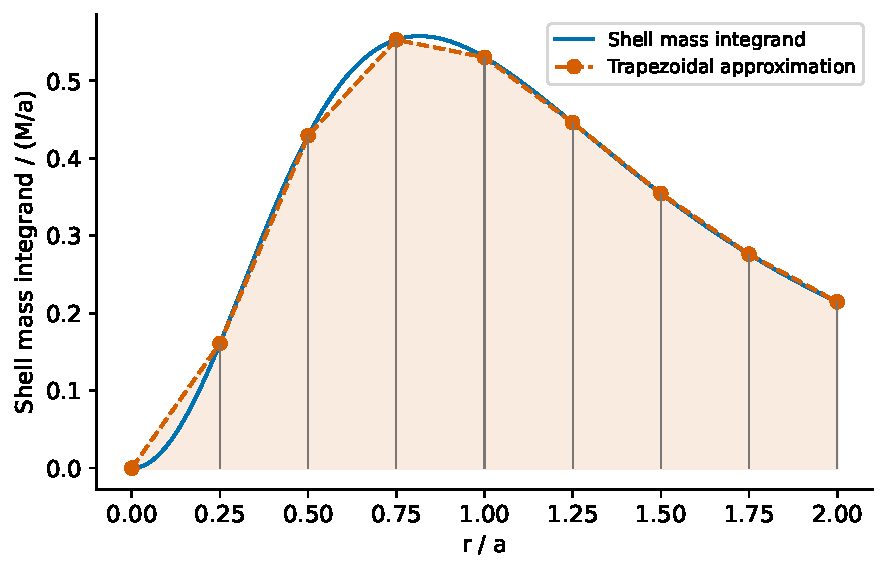
\includegraphics[width=118mm]{figures/ch03_trapezoid.pdf}};
  \begin{scope}[x={(plot.south east)},y={(plot.north west)}]
    \draw[figblue,line width=.85pt] (.645294,.181406) -- (.645294,.784836);
    \draw[figblue,line width=.85pt] (.744648,.181406) -- (.744648,.661074);
    \node[fill=white,inner sep=1.5pt,anchor=east,small label] (gl) at (.618,.64) {$g_j/(M/a)$};
    \draw[guide] (gl.east) -- (.645294,.770);
    \node[fill=white,inner sep=1.5pt,anchor=west,small label] (gr) at (.778,.48) {$g_{j+1}/(M/a)$};
    \draw[guide] (gr.west) -- (.744648,.645);
    \draw[{Latex[length=1.6mm]}-{Latex[length=1.6mm]},figblue] (.645294,.28) -- (.744648,.28);
    \node[small label,fill=white,inner sep=1pt,above] at (.694971,.29) {$\Delta r_j/a$};
  \end{scope}
\end{tikzpicture}

\caption{台形則で近似する球殻の質量の被積分関数。説明用に$0\leq r\leq2a$を8区間へ分けています。縦軸は$g/(M/a)=3(r/a)^2[1+(r/a)^2]^{-5/2}$です。標準の256区間の計算とは分割数が異なります。一つの台形の高さ$g_j,g_{j+1}$と幅$\Delta r_j$を注記しています。図の軸に合わせ、高さを$M/a$、幅を$a$で規格化しています。}
\label{fig:ch3-trapezoid}
\end{figure}

\subsection{各半径までの質量を順に足す}
すべての台形を最後に足すだけでなく、途中の和も保存します。数値積分で得た質量を$\widehat M_j$と書くと、
\begin{equation}
 \widehat M_0=0,\qquad
 \widehat M_{j+1}=\widehat M_j+\frac{g_j+g_{j+1}}{2}(r_{j+1}-r_j)
 \label{eq:ch3-cumulative-trapezoid}
\end{equation}
です。最後の値だけでなく、各分点に対応する累積質量の表が得られます。ハットはここでは数値近似を示すもので、無次元量を意味しません。

まずループで、式をそのまま実装します。
\inputcode{chap03/trapezoid}
\texttt{check\_grid}は、分点と関数値が同じ長さの1次元配列で、値が有限かつ分点が狭義単調増加していることを確認する補助関数です。実装はNotebookに置きます。積分の本体は、台形の面積を計算し、前の和へ足す2行です。

この関数へ、半径の表と$g$の値を渡します。
\inputcode{chap03/mass-table}
\texttt{mass\_numeric[j]}が$r_j$以内の質量です。\texttt{np.linspace}の最後の引数は分点数なので、区間数に1を加えます。

Notebookには、隣接する値をスライスで取り出し、\texttt{np.cumsum}で累積和を作る書き方も示します。計算している台形はループ版と同じです。まずは式と各配列要素の対応を理解し、コードが短いことだけを目標にしないようにします。

\subsection{2次精度の意味を確認する}
滑らかな関数について、一つの幅$\Delta r$の小区間を台形で近似した誤差は$O(\Delta r^3)$です。固定した範囲を等分すると、小区間の個数は$\Delta r^{-1}$に比例します。そのため、小区間の誤差を足した合成台形則の誤差は、通常$O(\Delta r^2)$になります。\cite{sugiura2009}

分割数を2倍にして幅を半分にすると、誤差がおよそ$1/4$になることを期待します。ただし、これは関数が滑らかで刻みが十分小さく、丸め誤差が支配しない範囲での話です。多項式を何次まで厳密に積分できるかという「代数的精度」とは、別の数え方です。本章では、\textbf{幅に対する誤差の変化}を確認します。

\begin{notebox}{ほかの数値積分法}
Simpson則は、小区間の関数を放物線で近似して積分する方法です。滑らかな問題では台形則より高い次数を得られます。Gauss求積のように、分点と重みの選び方を工夫する方法もあります。本章では、表から累積積分を作りやすい台形則を使います。ほかの方法の導出・実装は数値計算の教科書に譲ります。台形則とSimpson則の比較は、文献\cite{sugiura2009}の第3章を参照してください。
\end{notebox}

\Needspace{10\baselineskip}
\section{数値積分を解析式と比べる}
\label{sec:ch3-mass-check}
\subsection{原点でも使える誤差を定義する}
数値積分と解析式を同じ分点で比較します。原点では$M(<0)=0$なので、各半径の質量で割った相対誤差は使いません。球全体の質量$M$で規格化し、
\begin{equation}
 e_M=\max_{0\leq j\leq N_r}\frac{|\widehat M_j-M(<r_j)|}{M}
 \label{eq:ch3-mass-error}
\end{equation}
とします。これなら原点を含む表全体を、一つの基準で評価できます。

\begin{figure}[htbp]
\centering\includegraphics[width=0.72\linewidth]{\figpath{ch03_enclosed_mass}}
\caption{Plummer球の累積質量。灰色破線が解析式、青実線が$0\leq r\leq5a$を256区間で積分した結果です。両者はこの縮尺ではほぼ重なります。上の点線は球全体の質量であり、$5a$の内側だけでは到達しません。}
\label{fig:ch3-enclosed-mass}
\end{figure}

標準条件の最大誤差は$e_M=\chthreevalMassError$でした。図\ref{fig:ch3-enclosed-mass}がほぼ重なっても、この差は0ではありません。図の見た目とは別に、数値で確認することが必要です。

\subsection{積分範囲を固定して分割する}
ここでは$r_{\rm tab}=5a$を変えず、区間数$N_r$だけを増やします。
\inputcode{chap03/mass-convergence}
\begin{table}[htbp]
\centering
\caption{台形則の分割数試験。積分範囲は全行で$[0,5a]$です。$p_M$は前の行との誤差比から求めた推定次数で、最初の行には比較相手がありません。}
\label{tab:ch3-mass-convergence}
\begin{tabular}{rrrr}\toprule
$N_r$ & $\Delta r\ [\mathrm{kpc}]$ & $e_M$ & $p_M$ \\
\midrule
20 & 0.750000 & $5.87\times 10^{-3}$ & --- \\
40 & 0.375000 & $1.46\times 10^{-3}$ & 2.0037 \\
80 & 0.187500 & $3.76\times 10^{-4}$ & 1.9602 \\
160 & 0.093750 & $9.40\times 10^{-5}$ & 2.0014 \\
320 & 0.046875 & $2.35\times 10^{-5}$ & 2.0004 \\
\bottomrule\end{tabular}

\end{table}

推定次数は、第1・2章の時間刻みの試験と同様に、
\begin{equation}
 p_M=\frac{\log[e_M(\Delta r)/e_M(\Delta r/2)]}{\log2}
 \label{eq:ch3-mass-order}
\end{equation}
で求めます。表\ref{tab:ch3-mass-convergence}の最も細かい側では$p_M=\chthreevalMassOrder$となり、2次の収束を確認できます。最大誤差を取る分点の位置も分割数とともに変わるため、粗い側の推定次数が滑らかに2へ近づくとは限りません。

\begin{figure}[htbp]
\centering\includegraphics[width=0.70\linewidth]{\figpath{ch03_mass_convergence}}
\caption{半径方向の幅と質量誤差。点線は、最も細かい分割の実測値を通る傾き2の参照線です。実測点を当てはめて傾きを決めた線ではありません。}
\label{fig:ch3-mass-convergence}
\end{figure}

\subsection{積分範囲の効果と積分誤差を区別する}
同じ$[0,5a]$をいくら細かく分けても、得られるのは$M(<5a)$です。全質量$M$にはなりません。式\eqref{eq:ch3-mass-exact}から求めた、いくつかの範囲内の質量を表\ref{tab:ch3-cutoff}に示します。
\begin{table}[htbp]
\centering
\caption{有限半径の内側と外側の質量。すべて解析式の値です。範囲外にある質量と、有限刻みによる数値積分誤差を区別します。}
\label{tab:ch3-cutoff}
\begin{tabular}{rrr}\toprule
$r_{\rm tab}/a$ & $M(<r_{\rm tab})/M$ & 範囲外の質量$/M$ \\
\midrule
5 & 0.942866034 & 0.057133966 \\
10 & 0.985185337 & 0.014814663 \\
20 & 0.996261685 & 0.003738315 \\
\bottomrule\end{tabular}

\end{table}

例えば$5a$より外には、全質量の約5.7\%が残ります。これは台形則の失敗ではありません。全質量まで近づけたいときには積分範囲も広げます。ただし、区間数を固定したまま範囲だけ広げると、中心付近の分割が粗くなります。\textbf{範囲を広げることと、同じ範囲を細かく分けることは、別の操作です。}

\begin{failbox}{最後の値を無条件に全質量へそろえない}
\texttt{mass\_numeric[-1]}を$M$に合わせて表全体を再規格化すると、積分範囲の外の質量を内側へ配り直してしまいます。本章の$M$は無限遠まで含めた全質量です。有限半径で切断した別のモデルを作るときは、その定義を改めて示す必要があります。
\end{failbox}

\section{二分法で半質量半径を求める}
\label{sec:ch3-bisection}
\subsection{半径を未知数にする}
ここまでは半径を指定して、その内側の質量を求めました。次は、質量を指定して半径を求めます。\textbf{半質量半径}$r_h$は、球全体の質量の半分が入る半径です。
\begin{equation}
 M(<r_h)=\frac{M}{2}.
 \label{eq:ch3-half-definition}
\end{equation}

Plummerモデルでは、解析式を使って比較値も求められます。式\eqref{eq:ch3-mass-exact}を$M$で割って$1/2$と置き、両辺を$2/3$乗すると、
\[
 \frac{r_h^2}{r_h^2+a^2}=2^{-2/3}.
\]
これを$r_h$について整理すると、
\begin{equation}
 r_h=\frac{a}{\sqrt{2^{2/3}-1}}\simeq1.304766\,a
 \label{eq:ch3-half-exact}
\end{equation}
です。本章の$a=3\unit{kpc}$では$r_h=\chthreevalRhExact\unit{kpc}$です。今回も、この解析式だけで答えを出すのではなく、数値的な求め方を検証します。

\subsection{積分と求根を分ける}
二分法は、関数の値が0になる場所を探す\textbf{求根法}です。本章で計算する関数を
\begin{equation}
 F(r)=\frac{\widehat M(<r)}{M}-\frac12
 \label{eq:ch3-root-function}
\end{equation}
とします。$\widehat M$は台形則の結果です。$F<0$なら内側の質量が半分より少なく、$F>0$なら多いことを意味します。

先ほどの質量表は決まった分点の値だけを持っていますが、二分法ではその間の半径も試します。そこで本章では、\textbf{半径を試すたびに$[0,r]$を同じ区間数で積分し直す}実装にします。表の補間をまだ必要とせず、二分法が呼ぶ関数の意味を直接追えます。
\inputcode{chap03/mass-at-radius}

\texttt{enclosed\_mass\_trapezoid}は積分、\texttt{half\_mass\_residual}は求根する方程式を担当します。$r=0$なら積分値は0として返します。$r>0$では、区間幅は$r/N_r$です。求根の途中では$r$が変わるので、分割幅も変わります。

\subsection{符号の変わる区間を半分にする}
連続な関数$F$について、端点$r_L<r_U$で符号が異なれば、その間に少なくとも一つの根があります。Plummer球の真の累積質量は単調増加するので、半質量半径は一つです。標準の数値積分でも、$[0,5a]$の両端で$F(0)<0$、$F(5a)>0$になります。

まず中点を計算します。
\begin{equation}
 r_C=\frac{r_L+r_U}{2}.
 \label{eq:ch3-bisection}
\end{equation}
$F(r_C)$が$F(r_L)$と同符号なら、根は右半分にあるので$r_L\leftarrow r_C$とします。異符号なら左半分を残し、$r_U\leftarrow r_C$とします。これを繰り返すのが二分法です。導関数は必要ありません。\cite{sugiura2009}

根が残る側を選んでいるので、区間の幅は毎回半分になります。ただし、符号が変わるだけで十分なのは、関数がその区間で連続な場合です。不連続な発散点を挟んで符号が違っても、そこに根があるとは限りません。


% BEGIN TikZ addition: ch03_bisection
図\ref{fig:concept-ch3-bisection}で、端点と中点の符号から、次に残す半区間をたどってください。太い線の範囲が次の行の探索区間になります。
\begin{figure}[!htbp]
\centering
% Standard [0,5a] bracket: signs correspond to the chapter's half-mass function.
% r_* denotes the root of the function actually evaluated, not an error-free physical radius.
\begin{tikzpicture}[textbook diagram,x=1cm,y=1cm]
  \node[anchor=west,font=\sffamily\bfseries] at (0,1.10) {Bisection: retain the half that contains the sign change};
  \draw[guide] (3.153,0.65) -- (3.153,-4.65);
  \node[above,fill=white,inner sep=1pt] at (3.153,0.65) {$r_*$};
  \foreach \k/\y/\lo/\mid/\hi/\keepL/\keepU/\sign in {
    0/0/0/2.5/5/0/2.5/+,
    1/-1.25/0/1.25/2.5/1.25/2.5/-,
    2/-2.5/1.25/1.875/2.5/1.25/1.875/+,
    3/-3.75/1.25/1.5625/1.875/1.25/1.5625/+} {
    \node[anchor=east] at (.72,\y) {$k=\k$};
    \draw[figgray,dashed] ({1+1.65*\lo},\y) -- ({1+1.65*\hi},\y);
    \draw[figblue,line width=3pt] ({1+1.65*\keepL},\y) -- ({1+1.65*\keepU},\y);
    \foreach \p in {\lo,\hi} {\draw[line width=0.8pt] ({1+1.65*\p},{\y-.13}) -- ({1+1.65*\p},{\y+.13});}
    \fill[figred] ({1+1.65*\mid},\y) circle (2.4pt);
    \node[above,inner sep=3pt] at ({1+1.65*\lo},{\y+.12}) {$-$};
    \node[above,inner sep=3pt] at ({1+1.65*\mid},{\y+.12}) {$\sign$};
    \node[above,inner sep=3pt] at ({1+1.65*\hi},{\y+.12}) {$+$};
    \node[anchor=west,small label] at (9.85,\y) {$w_0/2^{\k}$};
  }
  \node[below] at (1,0) {$r_L$};
  \node[below] at (5.125,0) {$r_C$};
  \node[below] at (9.25,0) {$r_U$};
  \draw[vector,figgray] (1,-4.70) -- (9.6,-4.70) node[right] {$r/a$};
  \foreach \x in {0,1,2,3,4,5} {\draw ({1+1.65*\x},-4.64) -- ({1+1.65*\x},-4.77);\node[below,small label] at ({1+1.65*\x},-4.77) {\x};}
  \draw[figblue,line width=3pt] (0.35,-5.53) -- (1.1,-5.53);
  \node[anchor=west,small label] at (1.25,-5.53) {Keep this half};
  \draw[figgray,dashed] (5.65,-5.53) -- (6.4,-5.53);
  \node[anchor=west,small label] at (6.55,-5.53) {Discard this half};
  \node[small label,anchor=west] at (0.35,-6.10) {$+/-$: sign of $F$; dot: midpoint; $w_0=5a$.};
\end{tikzpicture}

\caption{初期区間$[0,5a]$からの二分法の例。点が中点、$+,-$が評価した$F$の符号、太い線が次に残す半区間です。$k$はそれまでの半減回数です。破線$r_*$は評価している数値関数の根であり、元の密度の真の半質量半径と必ずしも一致しません。}
\label{fig:concept-ch3-bisection}
\end{figure}
\FloatBarrier
% END TikZ addition: ch03_bisection

\subsection{二分法の終了条件を決める}
初期区間の幅を$w_0$とします。$k$回区間を半分にした後の幅は$w_k=w_0/2^k$です。その区間の中点を根の近似値とすれば、区間が正しい根を含む限り、中点から根までの距離は半区間幅以下です。
\begin{equation}
 |r_C-r_\ast|\leq\frac{w_k}{2}=\frac{w_0}{2^{k+1}}.
 \label{eq:ch3-root-bound}
\end{equation}
ここで$r_\ast$は、\textbf{実際に評価している関数$F$の根}です。まだ、元の連続的な密度の真の半質量半径$r_h$と同じとは限りません。

本章では、半区間幅が許容値$\tau_r$以下になったら終了します。$\tau_r$は半径と同じ単位を持ちます。例えば\texttt{root\_xtol = 1e-8}は$10^{-8}\unit{kpc}$です。無次元の残差$|F|$の許容値ではありません。

符号を保つ更新をコードにします。
\inputcode{chap03/bisection}

\texttt{check\_bisection}は、区間、許容幅、反復回数、端点の符号を確認します。\texttt{finite\_value}は、関数値が有限であることを確認します。両者の完全なコードはNotebookに含めます。\texttt{np.signbit}は負の符号を持つかどうかを返し、関数値どうしの積を作らずに同符号かを判定できます。

\texttt{trace}には、反復番号、左右の端点、中点、残差、半区間幅を保存します。関数値が計算上ちょうど0になった場合も終了します。通常の浮動小数点演算を使うため、これは丸めを含めて厳密に根を保証する区間演算の実装ではありません。更新が丸めの限界に達したときや反復上限を超えたときには、未収束として停止します。

\subsection{実際に半質量半径を求める}
\inputcode{chap03/half-mass}
標準の256区間では、数値結果は$\widehat r_h=\chthreevalRh\unit{kpc}$でした。区間を半分にした回数は\chthreevalRootHalvings 回、中点を評価した回数は\chthreevalRootCalls 回です。最初の区間の中点も評価しているため、二つの回数は1だけ異なります。終了時の半区間幅は$\chthreevalRootWidth\unit{kpc}$です。

\begin{notebox}{ほかの求根法}
Newton法は関数値と導関数から次の近似値を決め、適切な条件では二分法より速く収束しますが、初期値や関数の性質に注意が必要です。割線法は導関数の代わりに二つの点から傾きを見積もります。Brent法は区間を保つ操作と補間を組み合わせる方法です。本章では、根を挟む区間を追いやすい二分法に集中します。二分法、Newton法、割線法は文献\cite{sugiura2009}の第9章を参照してください。Brent法など、ここで扱わない方法の詳細は数値計算の専門書に譲ります。
\end{notebox}

\section{求根の残差と半径の誤差を区別する}
\label{sec:ch3-root-errors}
\subsection{二つの誤差を区別する}
二分法を終えたときの$|F(\widehat r_h)|$は$\chthreevalRootResidual$でした。一方、同じ半径を解析的な質量式へ代入したときの残差は、
\[
 \left|\frac{M(<\widehat r_h)}{M}-\frac12\right|=\chthreevalTrueResidual
\]
です。二つの値は一致しません。二分法は台形則で定義した$F$を0へ近づけていますが、その$F$自体に積分の誤差が含まれるためです。

実際、真の半径との差は$|\widehat r_h-r_h|=\chthreevalRhError\unit{kpc}$で、二分法の最終半区間幅より大きくなっています。式\eqref{eq:ch3-root-bound}が誤っているのではありません。そこに現れる$r_\ast$が、台形則で作った関数の根だからです。

\subsection{まず積分の分割数を変える}
求根の初期区間と許容幅を固定し、質量積分の区間数だけを変えます。
\inputcode{chap03/root-convergence}
\begin{table}[htbp]
\centering
\caption{積分の区間数による半質量半径の変化。二分法の許容半区間幅は全行で$10^{-8}\unit{kpc}$です。小さな数値残差が得られていても、真の半径との差には区間数への依存が残ります。}
\label{tab:ch3-root-convergence}
\small\begin{tabular}{rrrr}\toprule
$N_r$ & $\widehat r_h\ [\mathrm{kpc}]$ & $|\widehat r_h-r_h|\ [\mathrm{kpc}]$ & $|F(\widehat r_h)|$ \\
\midrule
32 & 3.914664479 & $3.66\times 10^{-4}$ & $7.95\times 10^{-10}$ \\
64 & 3.914389650 & $9.16\times 10^{-5}$ & $5.68\times 10^{-10}$ \\
128 & 3.914320974 & $2.29\times 10^{-5}$ & $3.60\times 10^{-10}$ \\
256 & 3.914303805 & $5.73\times 10^{-6}$ & $3.93\times 10^{-10}$ \\
512 & 3.914299516 & $1.44\times 10^{-6}$ & $8.84\times 10^{-10}$ \\
\bottomrule\end{tabular}

\end{table}

表\ref{tab:ch3-root-convergence}では、積分を細かくすると真の半径との差も小さくなります。本例では、その差はおよそ区間数の2乗に反比例して減っています。求根の終了条件を厳しくする前に、その関数値をどの精度で計算しているかを見る必要があります。

\subsection{次に求根の許容幅だけを変える}
今度は積分を64区間に固定し、$\tau_r$だけを変えます。
\begin{table}[htbp]
\centering
\caption{積分を64区間に固定した許容幅の試験。求根を細かく続けても、積分から来る半径のずれは取り除けません。}
\label{tab:ch3-root-tolerance}
\small\begin{tabular}{rrrr}\toprule
$\tau_r\ [\mathrm{kpc}]$ & 最終半区間幅$\ [\mathrm{kpc}]$ & 真の半径との差$\ [\mathrm{kpc}]$ & $|F|$ \\
\midrule
$1.00\times 10^{-2}$ & $7.32\times 10^{-3}$ & $4.16\times 10^{-3}$ & $5.76\times 10^{-4}$ \\
$1.00\times 10^{-4}$ & $5.72\times 10^{-5}$ & $9.63\times 10^{-5}$ & $6.70\times 10^{-7}$ \\
$1.00\times 10^{-6}$ & $8.94\times 10^{-7}$ & $9.18\times 10^{-5}$ & $3.61\times 10^{-8}$ \\
$1.00\times 10^{-8}$ & $6.98\times 10^{-9}$ & $9.16\times 10^{-5}$ & $5.68\times 10^{-10}$ \\
\bottomrule\end{tabular}

\end{table}

許容幅が十分小さくなると、真の半径との差は約$\chthreevalRootFloor\unit{kpc}$の付近でほぼ変わらなくなります。これは計算機の丸め誤差まで到達したからではなく、この実験では質量積分の誤差が残っているからです。

\begin{figure}[htbp]
\centering\includegraphics[width=0.73\linewidth]{\figpath{ch03_bisection_errors}}
\caption{64区間の質量積分を使った二分法の履歴。青は半区間幅、朱色は中点と解析的な半質量半径の差です。半区間幅は半減を続けますが、真の半径との差は積分誤差の大きさ付近に残ります。どちらも$a$で規格化しています。}
\label{fig:ch3-bisection-errors}
\end{figure}

\begin{failbox}{求根の桁数だけで結果の精度を判断しない}
数値的な関数の残差が小さくても、もとの方程式を同じ精度で解けたとは限りません。積分の分割数と求根の許容幅を別々に変更して確認します。また、$M/2$を$\widehat M(<r_{\rm tab})/2$へ替えると、有限の範囲内にある質量の半分を求める、別の問題になります。
\end{failbox}

\section{Plummer球の重力で星を動かす}
\label{sec:ch3-orbit}
\subsection{加速度は解析式から与える}
ここからは、星を表す1粒子の時間発展を計算します。質量積分と求根の誤差を軌道へ混ぜないため、\textbf{本章の標準軌道計算には解析的なPlummer加速度を使います。}数値的な質量表は、ここまでの積分・求根の学習と検証に使ったものです。

式\eqref{eq:ch3-potential}を微分すると、
\[
 \frac{d\Phi}{dr}=\frac{GM r}{(r^2+a^2)^{3/2}}
\]
なので、加速度は
\begin{equation}
 \boxed{\avec(\rvec)=-\frac{GM\rvec}{(r^2+a^2)^{3/2}}}
 \label{eq:ch3-acceleration}
\end{equation}
です。これは式\eqref{eq:ch3-enclosed-force}へ解析的な$M(<r)$を代入しても得られます。二つの求め方が一致することが、密度・質量・ポテンシャルの整合性の確認になります。

原点では$\avec=0$です。$r\ll a$では
\begin{equation}
 \avec\simeq-\frac{GM}{a^3}\rvec,
 \label{eq:ch3-inner-force}
\end{equation}
となり、位置に比例する調和振動子の形になります。一方、$r\gg a$では点質量の重力へ近づきます。中心で加速度が発散しないのは、質量分布を広げたモデルの性質であり、計算エラーを隠す処置ではありません。

\subsection{円運動速度も同じモデルから求める}
式\eqref{eq:ch3-vc-general}に代入すると、
\begin{equation}
 v_c^2(r)=\frac{GMr^2}{(r^2+a^2)^{3/2}},\qquad
 \Omega_c(r)=\frac{v_c(r)}{r}
 \label{eq:ch3-circular-speed}
\end{equation}
です。$r>0$の円軌道周期は$T_c(r)=2\pi/\Omega_c(r)$になります。中心近くでは$v_c\propto r$、十分外では$v_c\propto r^{-1/2}$です。\cite{bt2008}

\begin{figure}[htbp]
\centering\includegraphics[width=0.72\linewidth]{\figpath{ch03_circular_speed}}
\caption{同じ全質量を持つPlummer球と点質量の円運動速度。丸は本章の初期半径$r_0=2a$です。点質量の曲線は$r\geq0.5a$だけを示しています。原点に向かって発散する点質量の速度と、中心で0へ向かうPlummer球の速度は異なります。}
\label{fig:ch3-circular-speed}
\end{figure}

まずは成分で加速度を計算します。
\inputcode{chap03/acceleration-scalar}
本章の初期位置では$\avec\simeq(\chthreevalAccelX,0)\unit{kpc\,Gyr^{-2}}$です。この計算を短い関数にします。
\inputcode{chap03/acceleration-plummer}
\texttt{pos}と返り値は、1粒子なので形が\texttt{(1, 2)}です。多数の粒子への一般化は、第4章で行います。円運動速度の関数では、半径ごとの表を描けるよう配列も受け取ります。

\begin{failbox}{点質量の円運動速度を流用しない}
Plummer球の内部では、全質量$M$を使った$\sqrt{GM/r}$は円運動速度ではありません。力のモデルを変えたら、初期速度も同じモデルから計算し直します。$a$を変えて円軌道を比較するときも同様です。
\end{failbox}

\section{KDKで円軌道と非円軌道を計算する}
\label{sec:ch3-kdk}
\subsection{変える初期値を一つにする}
初期半径を$r_0=2a=6\unit{kpc}$とし、初期位置と速度を
\begin{equation}
 \rvec(0)=(r_0,0),\qquad \vvec(0)=(0,\eta v_c(r_0))
 \label{eq:ch3-initial}
\end{equation}
と置きます。$\eta=1$が円軌道、$\eta=0.7$が比較する非円軌道です。どちらも動径方向の初期速度は0で、反時計回りに動き始めます。

$0<\eta<1$では、円運動を保つために必要な接線速度より遅いため、初期半径から内側へ動き始めます。この初期位置は遠点です。ただし、第2章のKepler問題とは違い、その後の軌道は一般には閉じた楕円になりません。\textbf{非円軌道を最初から「楕円」と呼ばない}ようにします。

\inputcode{chap03/orbit-parameters}
\begin{table}[htbp]
\centering
\caption{本章の標準軌道条件。二つのケースで共通の基準周期$T_c$を使います。これは非円軌道の動径振動の周期を表す記号ではありません。}
\label{tab:ch3-parameters}
\begin{tabular}{ll}\toprule
量 & 設定または計算値\\\midrule
$M$, $a$ & $10^{11}\Msun$, $3\unit{kpc}$\\
$r_0$ & $6\unit{kpc}=2a$\\
$v_c(r_0)$ & $\chthreevalVc\unit{km\,s^{-1}}$\\
$T_c=2\pi r_0/v_c(r_0)$ & $\chthreevalTc\unit{Gyr}$\\
$\eta$ & $1$, $0.7$\\
$t_{\rm end}$ & $5T_c=\chthreevalTend\unit{Gyr}$\\
$N_{\rm step}$, $\Delta t$ & $5000$, $T_c/1000=\chthreevalDt\unit{Myr}$\\\bottomrule
\end{tabular}
\end{table}

初期状態を作る関数は、位置と速度を横につないだ\texttt{(1, 4)}の配列を返します。
\inputcode{chap03/initial-state}
\texttt{check\_model}は、$M$と$a$が有限かつ正であることを確認する関数です。KDKでは、まとめた状態から位置と速度を分けて取り出し、更新します。

\subsection{前章の積分法を再利用する}
KDKの計算は、半ステップの速度更新、1ステップの位置更新、新しい位置での加速度評価、残りの半ステップの速度更新です。
\inputcode{chap03/leapfrog-step}
前章から変えたのは、重力の関数へ渡すパラメータです。今回は二つの質量の配列ではなく、1個の銀河の\texttt{mass}と\texttt{a}を渡します。KDKの4行と、最後の加速度を再利用する構造は同じです。

\inputcode{chap03/integrate-leapfrog}
\texttt{prepare\_history}は、初期値をコピーし、時刻の配列と保存領域を作る補助関数です。前章と同じ役割ですが、今回は初期状態が\texttt{(1, 4)}であることを確認します。履歴は\texttt{(n\_steps + 1, 1, 4)}です。保存する速度は、最後の半ステップの更新を終えた整数時刻の値です。

5000ステップなら、加速度関数の評価は初回を含めて5001回です。台形則の区間数や二分法の反復回数は、この回数に含めません。いま評価している重力には解析式を使っています。

\subsection{同じ時間まで独立に計算する}
\inputcode{chap03/run-orbits}
一つのケースの最終状態を、別のケースの初期状態に流用しません。いずれも式\eqref{eq:ch3-initial}から作り直します。実行時間は環境に依存するので、Notebookで\texttt{perf\_counter}を使って測ります。

\begin{figure}[htbp]
\centering\includegraphics[width=0.70\linewidth]{\figpath{ch03_orbits}}
\caption{静的なPlummer球中の円軌道と非円軌道。青実線が$\eta=1$、朱色破線が$\eta=0.7$で、どちらも$5T_c$まで計算しています。中心の十字はポテンシャルの中心であり、追加した点質量ではありません。丸が共通の初期位置です。}
\label{fig:ch3-orbits}
\end{figure}

円軌道では半径がほぼ一定ですが、非円軌道では半径が増減し、近点・遠点の方向も変わります。このような軌道はロゼット軌道と呼ばれます。球対称でも、動径方向の振動と方位角方向の回転が、Kepler問題と同じ周期関係になるとは限りません。\cite{bt2008} 数値誤差による軌道のずれと区別するため、後で時間刻みを細かくした結果も比べます。

Notebookには、保存済みの履歴を使うアニメーションも含めます。画面上の再生間隔は物理的な時間刻みとは別で、動画の速度を変えても数値軌道は変わりません。

\Needspace{10\baselineskip}
\section{保存量と時間刻みを確認する}
\label{sec:ch3-validation}
\subsection{確認するエネルギーを決める}
固定した銀河ポテンシャル中のテスト粒子なので、確認するのは粒子の\textbf{単位質量当たり}のエネルギーと角運動量です。
\begin{equation}
 \varepsilon=\frac12(v_x^2+v_y^2)-\frac{GM}{\sqrt{r^2+a^2}},\qquad
 \ell_z=xv_y-yv_x.
 \label{eq:ch3-invariants}
\end{equation}
$\Phi$は時間に依存しないので、
\[
 \frac{d\varepsilon}{dt}=\vvec\cdot\avec+\nabla\Phi\cdot\vvec=0
\]
です。力は中心向きなので、$d\ell_z/dt=x a_y-y a_x=0$でもあります。第2章の二つの質量を掛けた全エネルギーや、Plummer球自身の自己重力エネルギーを計算しているわけではありません。

\inputcode{chap03/diagnostics}
位置と速度を同じ保存時刻から取り出します。Plummerポテンシャルを使って運動した結果に、点質量の$-GM/r$を足してエネルギーを診断しないようにします。

\subsection{有限刻みによる差を測る}
今回の2例では$\varepsilon(0)$と$\ell_z(0)$がともに0ではないので、その絶対値で規格化できます。保存した全時刻での最大値を
\begin{equation}
 e_\varepsilon=\max_n\frac{|\varepsilon^n-\varepsilon^0|}{|\varepsilon^0|},\qquad
 e_\ell=\max_n\frac{|\ell_z^n-\ell_z^0|}{|\ell_z^0|}
 \label{eq:ch3-invariant-errors}
\end{equation}
とします。初期値が0の別の軌道では、この規格化は使わず、第2章のように正の基準量を選ぶ必要があります。

\begin{table}[htbp]
\centering
\caption{標準条件の保存量と最小保存半径。両例とも$5T_c$まで5000ステップで計算しています。角運動量の末尾の桁は実行環境で多少変わります。}
\label{tab:ch3-conservation}
\small\begin{tabular}{lrrr}\toprule
軌道 & $e_\varepsilon$ & $e_\ell$ & 保存された最小半径$\ [\mathrm{kpc}]$ \\
\midrule
円 & $1.62\times 10^{-10}$ & $1.08\times 10^{-14}$ & 6.000000 \\
非円 & $1.83\times 10^{-5}$ & $9.47\times 10^{-15}$ & 3.027208 \\
\bottomrule\end{tabular}

\end{table}

\begin{figure}[htbp]
\centering\includegraphics[width=0.73\linewidth]{\figpath{ch03_energy}}
\caption{粒子の比エネルギーの初期値からの符号付きの差。円軌道の差は小さく、この縮尺では0付近に重なります。非円軌道では半径の増減に伴い差が変動します。これは摩擦によるエネルギー損失を入れた計算ではありません。}
\label{fig:ch3-energy}
\end{figure}

KDKでは中心力によるkickも、速度を固定するdriftも角運動量を保つため、$e_\ell$は丸め誤差程度になります。一方、エネルギーを毎ステップ厳密に保つ方法ではないので、円軌道では$e_\varepsilon=\chthreevalCircEnergy$、非円軌道では$\chthreevalNoncEnergy$という有限の差が現れました。保存量が小さくずれることと、軌道上の位置が同じ精度で正しいことは、別に調べます。

\subsection{円軌道を同じ時刻の解析位置と比べる}
円軌道では、$\Omega_c=v_c(r_0)/r_0$から解析的な位置を
\begin{equation}
 \rvec_{\rm exact}(t)=r_0(\cos\Omega_c t,\sin\Omega_c t)
 \label{eq:ch3-circle-exact}
\end{equation}
と書けます。同じ時刻の数値解との最大の距離を、初期半径で規格化します。
\begin{equation}
 e_r=\max_n\frac{|\rvec^n-\rvec_{\rm exact}(t_n)|}{r_0}.
 \label{eq:ch3-position-error}
\end{equation}
半径の差だけではないので、回転の位相がずれた場合も検出できます。

この試験だけ最終時刻を$T_c$とし、100、200、400、800ステップで比較します。$5T_c$の標準図とは計算時間が異なりますが、試験系列の中では同じ時刻まで計算します。
\inputcode{chap03/orbit-convergence}

\begin{table}[htbp]
\centering
\caption{Plummer球中の円軌道の時間刻み試験。最終時刻は全行で解析的な円軌道周期$T_c$です。$p_r$は前の行との位置誤差の比から求めます。}
\label{tab:ch3-orbit-convergence}
\begin{tabular}{rrrr}\toprule
$N_{\rm step}$ & $\Delta t\ [\mathrm{Myr}]$ & $e_r$ & $p_r$ \\
\midrule
100 & 1.627630 & $3.25\times 10^{-3}$ & --- \\
200 & 0.813815 & $8.12\times 10^{-4}$ & 2.00052 \\
400 & 0.406907 & $2.03\times 10^{-4}$ & 2.00020 \\
800 & 0.203454 & $5.07\times 10^{-5}$ & 2.00005 \\
\bottomrule\end{tabular}

\end{table}

\begin{figure}[htbp]
\centering\includegraphics[width=0.72\linewidth]{\figpath{ch03_orbit_convergence}}
\caption{Plummer球中の円軌道に対する位置誤差。横軸は$\Delta t/T_c$です。点線は、最も細かい刻みの実測点を通る傾き2の参照線です。}
\label{fig:ch3-orbit-convergence}
\end{figure}

最も細かい側の推定次数は$p_r=\chthreevalOrbitOrder$で、KDKの2次精度を確認できました。重力場を点質量からPlummer球へ変えても、滑らかな軌道を十分小さい刻みで追う場合の次数は同じです。円軌道のエネルギー誤差には特殊な打ち消しが生じる場合があるので、その誤差だけから解法の次数を判断しません。

\subsection{閉じない非円軌道の精度を確かめる}
非円軌道では、$T_c$や$5T_c$後に初期位置へ戻るとは限りません。初期位置へ戻らない量を、そのまま誤差にしてはいけません。本章では、同じ$5T_c$まで異なる刻みで計算した終点を比較します。

刻み$h$と$h/2$による終点を使い、
\begin{equation}
 d_h=\frac{|\rvec_h(t_{\rm end})-\rvec_{h/2}(t_{\rm end})|}{r_0}
 \label{eq:ch3-self-convergence}
\end{equation}
とします。もし$\rvec_h=\rvec_{\rm true}+\boldsymbol C h^2+\cdots$で主要な誤差を表せるなら、差を取ると$(3/4)\boldsymbol C h^2$が残るので、$d_h/d_{h/2}$は約4になります。

\begin{table}[htbp]
\centering
\caption{非円軌道の終点の自己収束試験。すべて$5T_c$まで計算します。各行は、隣接する二つの刻みの数値解の差です。真の解との誤差ではありません。}
\label{tab:ch3-noncircular}
\small\begin{tabular}{rrrr}\toprule
粗い計算のステップ数 & 細かい計算のステップ数 & 終点の差$/r_0$ & 前の行との比 \\
\midrule
1250 & 2500 & $8.98\times 10^{-4}$ & --- \\
2500 & 5000 & $2.25\times 10^{-4}$ & 3.99969 \\
5000 & 10000 & $5.61\times 10^{-5}$ & 3.99992 \\
\bottomrule\end{tabular}

\end{table}

細かい側の比は\chthreevalNoncRatio で、およそ4でした。図\ref{fig:ch3-orbits}のロゼット状の運動が、刻みを細かくするとKepler楕円へ変わるわけではありません。ただし、自己収束の確認だけで、力の式そのものが正しいと証明できるわけでもありません。解析的な円軌道、密度と力の関係、保存量と合わせて判断します。

\section{三つの数値計算の役割を区別する}
\label{sec:ch3-error-budget}
ここまでの計算では、同じPlummerモデルに対して、異なる目的の算法を使いました。どの入力を変えると、どの誤差を調べることになるかを整理しておきます。

\begin{center}
\begin{tabularx}{\linewidth}{lXX}\toprule
操作 & 固定するもの & 確認するもの\\\midrule
台形則の区間を細かくする & 積分範囲、密度モデル & 解析的な質量との差\\
二分法の許容幅を小さくする & 質量積分の区間数、求根区間 & 数値的な関数の根の精度\\
KDKの時間刻みを小さくする & 初期条件、重力場、最終時刻 & 軌道位置と保存量の変化\\\bottomrule
\end{tabularx}
\end{center}

$a$を変えることは、これらの数値精度を調整することとは違います。密度分布と重力そのものを変更する、\textbf{物理モデルの変更}です。例えば$M$と$r_0$を固定して$a$を大きくすると、内側の質量が減り、円運動速度は小さくなります。円軌道を比較するのか、同じ位置・速度から異なるポテンシャルでの応答を比べるのかによって、そろえる初期条件も変わります。

また、本章では軌道に解析的な力を使っているので、台形則の区間数を変えても、そのまま軌道の計算結果が変わることはありません。数値的な質量表から力を計算する実装へ拡張した場合には、空間の積分・補間誤差と時間積分誤差を、改めて分けて確かめる必要があります。そこまでの拡張は本章の必須課題にはしません。

\section{本章のまとめ}
\label{sec:ch3-summary}
本章では、質量に広がりを持つ静的な銀河を、球対称のPlummerモデルで表しました。密度を球殻の体積で重み付けして積分すると、内側の質量が得られます。球対称の重力加速度と円運動速度は、その内側の質量から決まります。一方、ポテンシャルには外側の質量も寄与するため、力と同じ置き換えを無条件に行いません。

台形則では、小区間の両端を結ぶ直線の下の面積を足しました。積分範囲を固定して幅を半分にすると、質量の誤差がおよそ$1/4$になることを確認しました。二分法では、半質量半径を挟む区間を保って半分にしました。ただし、二分法の残差を小さくしても、関数値に含まれる質量積分の誤差までは消えません。

最後に、解析的なPlummer加速度をKDKへ渡して、円軌道と非円軌道を計算しました。固定した球対称場では、粒子の比エネルギーと比角運動量を確認できます。円軌道の解析位置と、非円軌道の刻みを変えた比較も使い、保存量だけに頼らず結果を確かめました。

次の第4章では、1個のテスト粒子から多数の粒子へ進みます。円盤上の分布を作るために、台形則による累積積分を再利用し、線形補間と乱数を組み合わせます。見た目に円盤状の粒子を配置しても、その粒子自身の自己重力を計算するわけではない、という区別を引き継ぎます。

\chapterexercises
\paragraph{演習3.1　確認：密度・質量・円運動速度}
$M=10^{11}\Msun$、$a=3\unit{kpc}$について、中心密度$\rho(0)$、$M(<a)/M$、半質量半径$r_h$を計算してください。また、$r=2a$での円運動速度を$\mathrm{km\,s^{-1}}$と内部単位の両方で示してください。軌道を2次元で計算する場合でも、質量積分に$4\pi r^2$が必要な理由を説明してください。

\paragraph{演習3.2　確認：台形則の配列}
$[0,5a]$を$N_r=40$区間に分けたときの分点数と区間幅を求めてください。\texttt{cumulative\_trapezoid}のループで、\texttt{integral[j + 1]}が何を表すか説明してください。密度ではなく$g=4\pi r^2\rho$を渡す理由を、単位からも確かめてください。

\paragraph{演習3.3　応用：範囲と分割数を分ける}
$[0,5a]$の区間数を増やす実験と、$\Delta r$を固定して範囲を$5a,10a,20a$へ広げる実験を行ってください。数値積分の誤差と範囲外の質量を別々に示してください。全質量$M$と$M(<5a)$の違いを、台形則の誤差だけで説明できるでしょうか。

\paragraph{演習3.4　確認：二分法の反復回数}
初期区間を$[0,15]\unit{kpc}$としたとき、半区間幅を$10^{-8}\unit{kpc}$以下にするには何回の半減が必要か求めてください。半減回数と中点評価回数の違いも示してください。また、$|F(\widehat r_h)|$が小さくても、$|\widehat r_h-r_h|$が同じ程度には小さくならない理由を説明してください。

\paragraph{演習3.5　応用：球全体の半分と、範囲内の半分}
求根式の右辺を$M/2$から$M(<5a)/2$へ変えて、二つの半径を比較してください。先に解析式で違いを確認し、その後、数値積分で作る関数を二分法で解いてください。どちらが小さくなるでしょうか。この変更が単なる数値精度の改善ではない理由を述べてください。

\paragraph{演習3.6　応用：スケール長を変える}
$M$と$r_0=6\unit{kpc}$を固定し、$a=1.5,3,6\unit{kpc}$の円運動速度と半質量半径を求めてください。それぞれに対応する円運動速度で初期条件を作り、円軌道を計算してください。すべてに同じ初期速度を与えた場合とは、何を比較している点が違うでしょうか。

\paragraph{演習3.7　発展：非円軌道の近点を求根で調べる}
$\eta=0.7$の初期比エネルギー$\varepsilon_0$、比角運動量$\ell_{z,0}$を用いて、
\begin{equation}
 \Phi(r)+\frac{\ell_{z,0}^2}{2r^2}-\varepsilon_0=0
 \label{eq:ch3-turning-point}
\end{equation}
の根を二分法で求めてください。この式は、動径速度が0になる条件です。初期遠点$r_0$ではない内側の根を探すため、区間を$[0.05r_0,0.95r_0]$とします。関数の符号を確認してから求根し、軌道の保存された最小半径と比較してください。両者の違いには何が含まれるでしょうか。
